\documentclass[
  manuscript=article,  %% article (default), rescience, data, or software
  layout=publish,  %% preprint (for submission) or publish (for publisher only)
  year=2023,
  volume=1,
]{extra/joas}

% --- blew is the area for authors ---


\usepackage[german]{babel}
\usepackage{graphicx}
% \usepackage{epstopdf, epsfig}
\graphicspath{ {imgs/} }
\usepackage[german]{babel}
\usepackage{hyperref} 
\usepackage{amsmath}
\usepackage{blindtext}
\usepackage{titlesec}
\usepackage{amsbsy}
\usepackage{caption}

% specify the .bib file for references
\addbibresource{reference.bib} 

% Make sure your article tile is within 12 words
\title{Das Meistern von chinesischem Schach mit autodidaktischem Reinforcement Learning}

\author{Simon Ma (15)}
\affiliation{Schillerschule Hannover, Ebellstr. 15, 30629 Hannover, Germany}
\email{simon.ma@iserv-schillerschule.de}

\begin{document}
\begin{abstract}
    Xiangqi, chinesisches Schach, ist ein unvorstellbar komplexes Spiel, dessen Meisterung Jahrzehnte dauert - für einen Menschen. CheapChess ist meine Xiangqi-Applikation, mit Fokus auf einer selbstlernenden KI, die sich um die Frage dreht, wie sich die ressourcenintensiven existierenden Programme optimieren und sich komplexe Probleme kostengünstig lösen lassen. Zentrale Schwerpunkte lagen neben der Entwicklung eines funktionsfähigen Xiangqi Environments vor allem auf dem Entwurf und der Optimierung eines autodidaktischen Reinforcement Learning Algorithmus und dessen Erweiterung mit einem hochperformanten Suchalgorithmus, alles mit limitierter Hardware. Dafür entwarf ich neue Konzepte und es entstand eine flexibler, starke Spiel-KI.
\end{abstract}

\begin{tabular}{l p{12cm}}

    Projektbetreuerin: & Birgit Ziegenmeyer                                                    \\

    Institution:       & Schillerschule Hannover                                               \\

    Thema des Projektes:
                       & Die Entwicklung eines autodidaktischen Reinforcement Learning 

    Algorithmus erweitert mit einem hochperformanten Suchalgorithmus um chinesisches Schach 
    zu meistern                                                                                \\

    Fachgebiet:        & Mathematik/Informatik                                                 \\

    Wettbewerbssparte: & Jugend Forscht                                                        \\

    Bundesland:        & Niedersachsen                                                         \\

    Wettbewerbsjahr:   & 2023                                                                  \\
\end{tabular}

\newpage

\begin{figure}
\centering
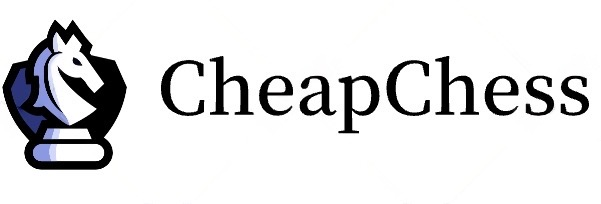
\includegraphics[width={0.5\textwidth}]{imgs/loogo.jpg}
\end{figure}
\maketitle

\tableofcontents

\newpage
\section{Einleitung}\label{sec:einleitung}
Bereits für die Väter der Informatik wurde Computer Schach zur Herausforderung. Babbage, Turing und Shannon entwickelten schon in den frühen 1950ern Algorithmen und Hardware, um das menschliche Verständnis über die Domäne auszubauen. Schach wurde schnell zu einer der größten Herausforderungen für Generationen von Forschern der künstlichen Intelligenz. 

Die meisten Schach-Programme, z.B. Stockfish, basieren dabei auf einer Kombination von hocheffizienten Suchalgorithmen, domänenspezifischen Optimierungen und handgefertigten Evaluationsfunktionen, welche Jahre lang von Experten optimiert wurden. 

Mit Deepminds AlphaZero führten 2017 innovative Konzepte und scheinbar unendliche Ressourcen zu einem der größten Durchbrüche in der KI-Forschung. Denn anstelle der herkömmlichen Evaluationsfunktionen lernte ein Convolutional Neural Network mithilfe eines raffinierten Reinforcement Learning allein durch Spiele gegen sich selbst Schach, Shogi und Go und schlug in jedem Spiel den jeweilige Weltmeister. Nur ist das Programm nicht öffentlich zugänglich und wohl kaum jemand besitzt die 5000+ Tensor Processing Units (TPUs), die Deepmind zur Verfügung standen. 

Das grundsätzliche Ziel von CheapChess ist die Entwicklung eines flexiblen und anpassbaren Trainingspartners, die Förderung von Zugänglichkeit zu innovativen Konzepten wie AlphaZero und die dafür benötigte Anpassung benötigter Ressourcen auf normale Konsumenten. Anders als Stockfish und AlphaZero fokussiere ich mich dabei jedoch spezifisch auf Xiangqi (chinesisches Schach). Xiangqi erfordert wegen seiner extremen Komplexität besondere Achtung auf Effizienz und durfte noch keine intensive Forschung genießen.

So entwarf ich eine Python Xiangqi Applikation und entwickelte einen effizienten selbstlernenden Reinforcement Learning Algorithmus ergänzt von hochoptimierten Such-Algorithmen. Ich erschuf eine Kombination aus den innovativen Konzepten von AlphaZero und den traditionellen Methoden von Stckfish, die beim Training beobachtet und zum Spielen herausgefordert werden kann. 

Meine Arbeit soll einerseits eine radikale Reduktion der benötigten Hardware ermöglichen, andererseits den Stärken einer Methode erlauben, für die Schwächen der anderen zu kompensieren und darüber hinaus zu neuen Einblicken in die taktische Welt von Xiangqi führen.

Xiangqi, auch bekannt als chinesisches Schach, ist ein strategisches Brettspiel, das tief in der chinesischen Kultur verwurzelt ist und seit dem neunten Jahrhundert überall in China gespielt wird. Seinen historischen Ursprung findet das Spiel schon um 200 v.Chr. , als sich zwei Dynastien vor einem der bedeutendsten Kämpfe der chinesischen Geschichte gegenüberstanden. Die Figuren sollen die zwei Armeen darstellen und der horizontale Barren in der Mitte des Feldes ist ein Symbol für den Fluss, der die Armeen auf dem Schlachtfeld trennte. 

\begin{figure}
  \centering
  \begin{minipage}{0.49\textwidth}
    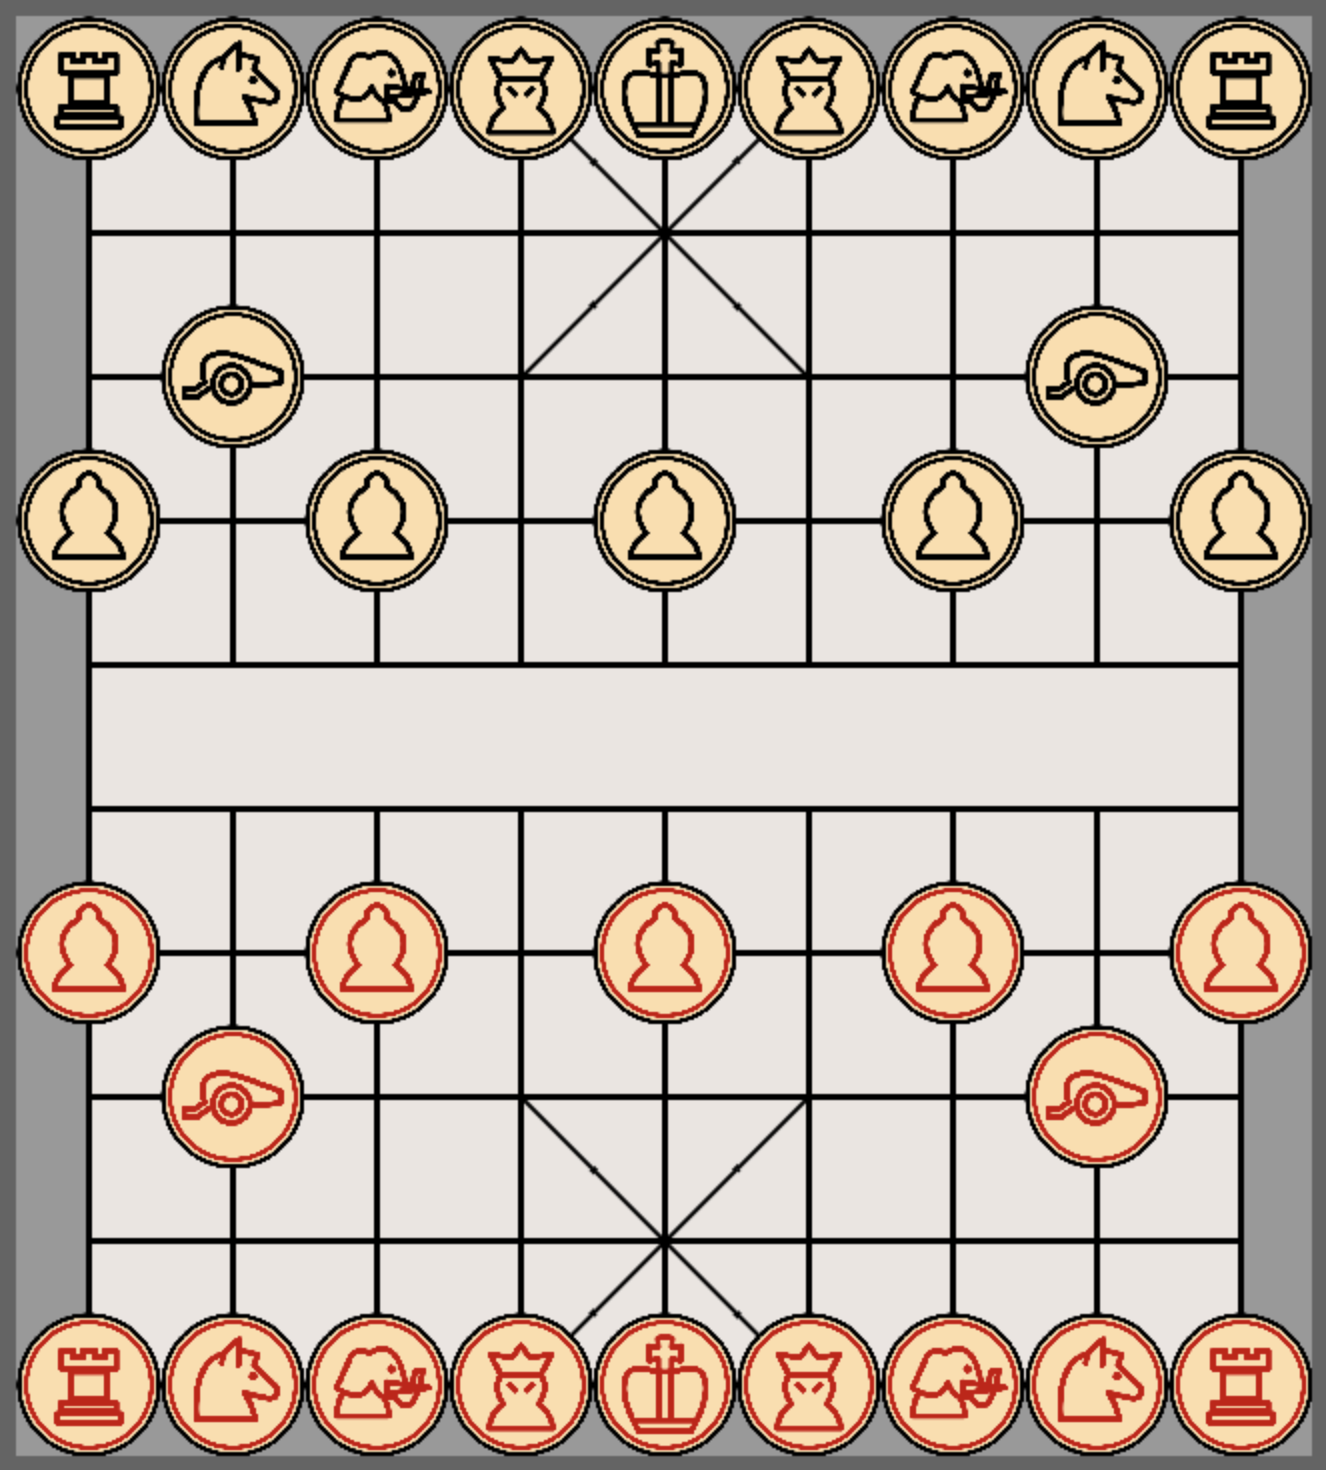
\includegraphics[width=\textwidth]{imgs/board.png}
  \end{minipage}
  \hfill
  \begin{minipage}{0.49\textwidth}
    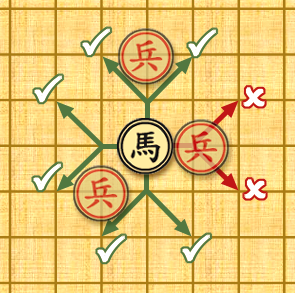
\includegraphics[width=\textwidth]{imgs/MovementOfHorsePiece.png}
    \caption{Züge des Pferdes}
  \end{minipage}
  \captionsetup{justification=centering}
  \caption{Die Standardaufstellung eines Xiangqi-Spiels, veranschaulicht mit dem GUI meiner Applikation (links)
  Züge des Pferdes (rechts)}
  \label{fig:horseandBoard}
\end{figure}
\section{Einführung zu Xiangqi}\label{sec:introtoxiangqi}
Das Spiel ist in einigen Aspekten ähnlich wie Schach, weist aber auch Unterschiede auf. So wird es auf einem $9 \times 10$ Brett gespielt und es gibt andere Figuren.
Das Brett besteht aus $9 \times 10$ Linien und Figuren stehen auf den Kreuzungen dieser Linien statt auf den Feldern. Um dem König herum ein Palast, welcher mit zusätzlichen Linien markiert ist \ref{fig:horseandBoard}.


Der Feldherr / König geht immer nur einen Schritt waagerecht oder senkrecht. Er darf den Palast nie verlassen und eine Rochade gibt es nicht. Die beiden gegnerischen Feldherren dürfen sich niemals ohne einen dazwischen stehenden Stein auf einer Linie gegenüberstehen. Der „Todesblick“ der Feldherrn verbietet dies, was besonders im Endspiel genutzt werden kann, um ein Patt (in Xiangqi kein Remis, sondern ein Sieg) zu erzwingen.

Die Leibwächter / Berater gehen immer nur einen Schritt diagonal auf ein unmittelbar benachbartes Feld und dürfen den Palast ebenfalls nicht verlassen. Somit stehen beiden zusammen nur fünf Felder zur Verfügung, nämlich die Palastmitte und dessen vier Ecken.

Die Elefanten gehen genau zwei Schritte in diagonaler Richtung. Falls das zwischenliegende (übersprungene) Feld besetzt ist, wird der Zug geblockt. Darüber hinaus dürfen die Elefanten niemals den Fluss überqueren.

Die Pferde entsprechen im Wesentlichen den Springern des internationalen Schachs, können jedoch ebenfalls blockiert werden. Ein Pferd bewegt sich in seinem Zug in zwei Schritten: zuerst ein Feld waagerecht oder senkrecht in beliebiger Richtung und anschließend ein Feld diagonal. Das Pferd wird blockiert, wenn eine andere Figur auf dem zuerst zu betretenden Feld steht \ref{fig:horseandBoard}.

 Der Turm / Wagen entspricht der den Türmen des europäischen Schachs. 
 
 Die Kanonen gibt es in internationalem Schach nicht. Wenn sie nicht schlagen, bewegen sie sich wie der Wagen. Zum Schlagen muss sich irgendwo zwischen dem gegnerischen Stein, und der Kanone genau ein anderer Stein befinden (Schanzenstein), der beim Schlagen übersprungen wird.
 
 Die Soldaten / Bauer bewegen sich ein Feld nach vorne und können nicht zurückgehen. Anders als Bauer im internationalen Schach können sie aber nach Überquerung des Flusses ein Feld seitlich ziehen und schlagen nicht diagonal, sondern im herkömmlichen Zugmuster (senk- und waagerecht)

\section{Xiangqi-Engine}
\begin{figure}
    \centering
    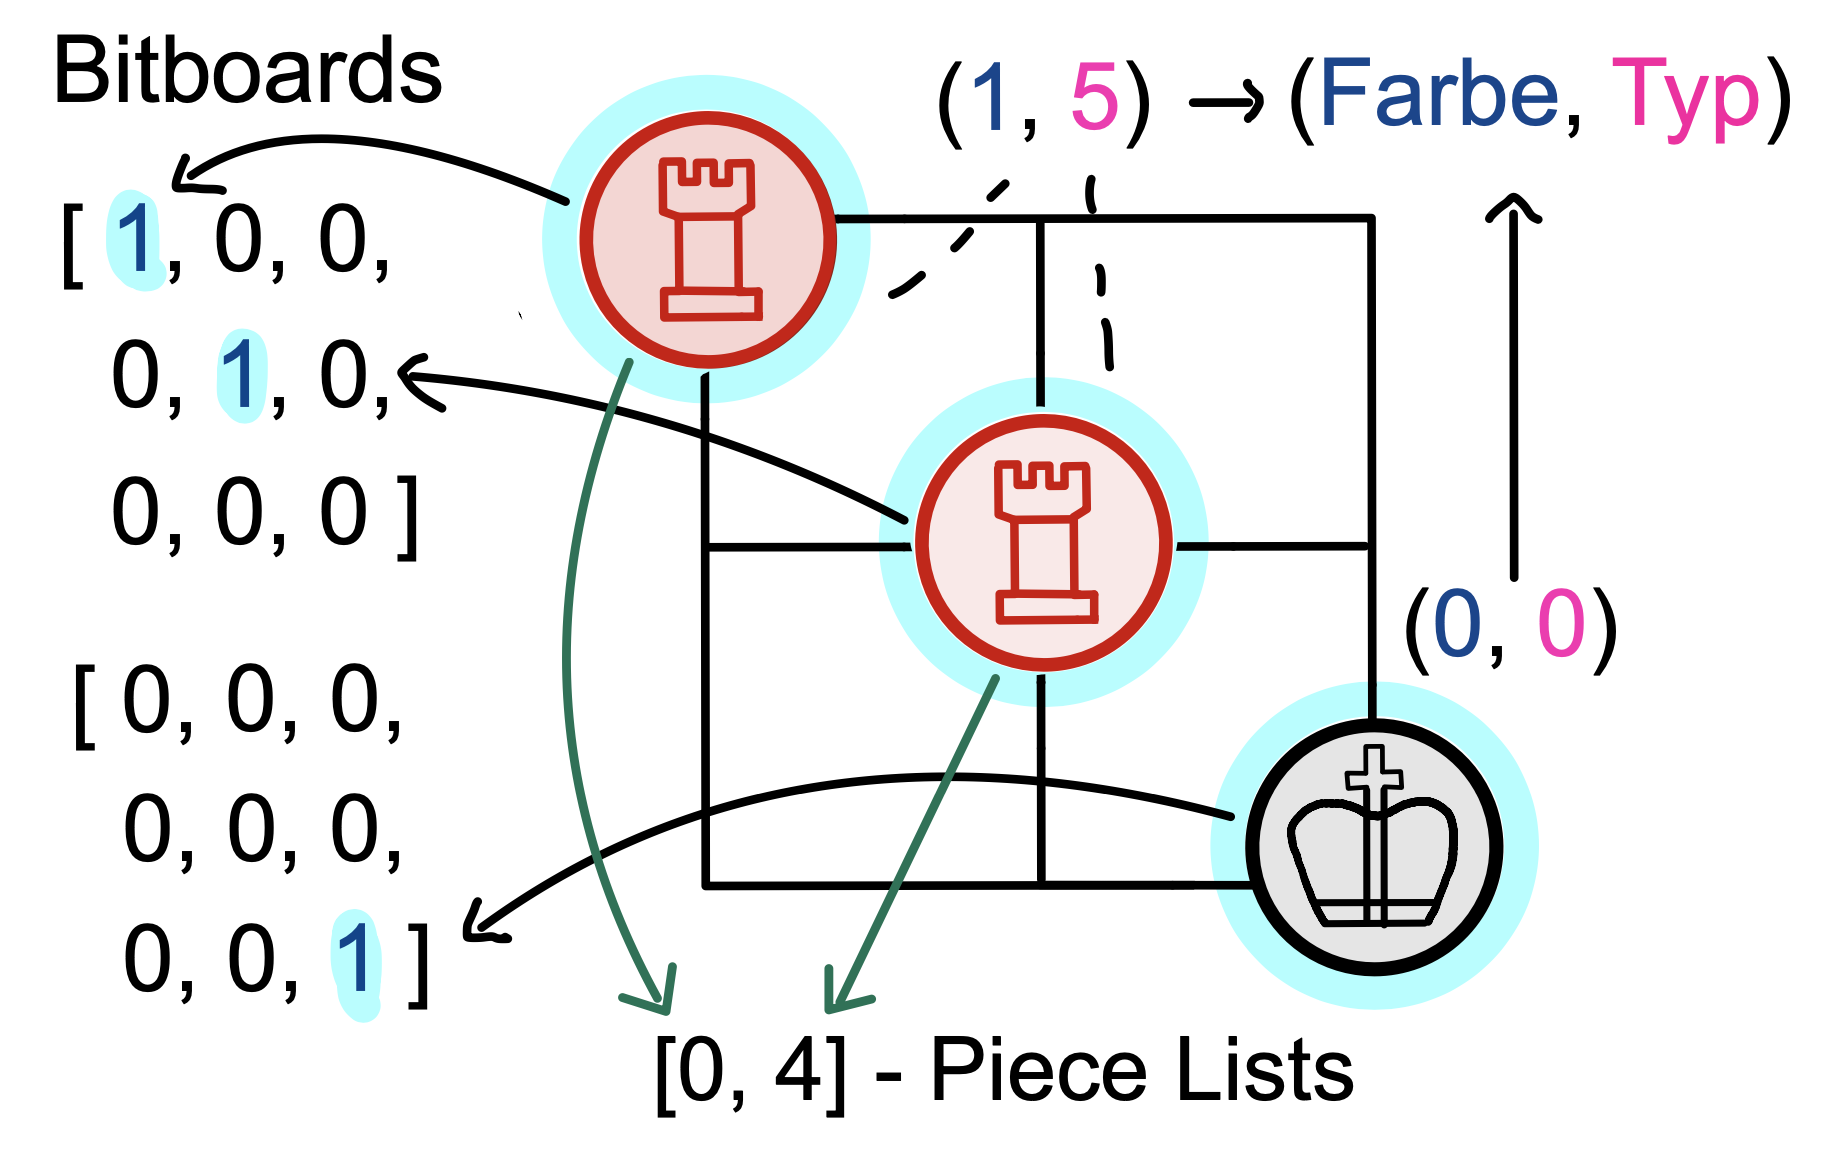
\includegraphics[width={0.6\textwidth}]{imgs/Board repr.png}
    \caption{Simplifizierte Visualisierung der internen Brettrepräsentation. Die Bitboards sind }
    \label{fig:repr}
\end{figure}
\subsection{Interne Brettdarstellung}\label{subsec:interneDarstellung}
Die interne Brettdarstellung ist die möglichst effiziente Repräsentation des Spiels im Code. Die Figuren werden als Tupel repräsentiert, wobei Index 0 die Farbe und Index 1 den Typ bestimmt. Die darstellung als 5-bit Zahl funktionierte, erwies sich aber als deutlich langsamer. Das Brett ($9\times10$) wird in drei verschiedenen Weisen dargestellt:

\begin{enumerate}
\item Feldzentrisch als ein-dimensionale Liste mit Länge 90 für 90 Felder, 0 für leeres Feld, Tupel für Figur (intuitivste Darstellungsform).
\item Figurenzentrisch als Liste der besetzten Felder für jeden Figurentyp jeder Farbe \ref{fig:repr}. 
\item Als Bitboard für jeden Figurentyp jeder Farbe. Bitboards sind binäre Repräsentationen des Bretts, wobei eine 0 für ein leeres und eine 1 für ein besetzt Feld steht \ref{fig:repr}. Ich nutze sie als Eingabe für mein Neuronales Netzwerk.
\item Forsyth-Edwards-Notation (FEN) für das Laden eines Spielzustandes von einem string
\item Zobrist-Hash-Key für die Kodierung des Spielzustandes in einen 8 Byte Integer
\end{enumerate}

  
\subsection{Zobrist-Hashing und LaZo}{\label{subsec:Zobrist}}
Für die folgenden KI-Suchalgorithmen ist es sehr wichtig, Spielzustände einfach und effizient darzustellen, z.B. für den schnellen Zugriff auf positionsspezifische Daten in einer Hash-Table. Ich fand heraus, dass der \textit{Zobrist-Hashing} Algorithmus die Kodierung eines Spielzustands in einen einzigen n-Bit Integer ermöglicht. \ref{fig:zobristVisLaZo} Ich wählte für die Größe des Hash-Schlüssels 64 Bits.
Aufgrund der  $2^{64}$ möglichen individuellen Hash-Werten sind Hash-Kollisionen besonders unwahrscheinlich, was Zobrist-Hashing zu einer sehr zuverlässigen Methode macht.

 \begin{figure}
    \centering
    \begin{minipage}{0.44\textwidth}
      \includegraphics[width=\textwidth]{imgs/zobristVis.png}
    \end{minipage}
    \hfill
    \begin{minipage}{0.49\textwidth}
      \includegraphics[width=\textwidth]{imgs/zobristVsLazo.png}
    \end{minipage}
    \captionsetup{justification=centering}
    \caption{Simplifizierte Zobrist Hashing Visualisierung Bezug auf \ref{fig:repr} (rechts) \\ Unterschiedliche Vorgehensweisen von Zobrist Hashing vs. Lazy-Zobrist (links)}
    \label{fig:zobristVisLaZo}
  \end{figure}
  
Um Zobrist Hashing für Xiangqi zu implementieren, werden vorerst Zobrist-Tabellen initialisiert. Diese besteht aus Zufallszahlen für jede Farbe, jede Figur und jedes Feld. Dargestellt habe ich sie als dreidimensionales numpy-array bestehend aus zufälligen 8-Byte Integern. 
Danach werden die jeweilgen Werte in den Zobrist-Tabellen für jede Figur auf dem Brett mit die bitweisen XOR-Operation (Kontravalenz) verkettet. Die sich bewegende Seite wird ebenfalls berücksichtigt.
Die Grundidee des Hashing-Algorithmus ist also die Abstrahierung der Merkmale des Bretts (mithilfe der Zufallszahlen der Zobrist-Tabellen) und die Nutzung dieser abstrakten Merkmale, um einen Hash-Schlüssel zu generieren.
  
Ich merkte hierbei, dass für die Generation des Hash-Schlüssels jedes mal über alle Figuren iteriert werden muss, obwohl sich für jeden Zug maximal die Position von zwei Figuren (\textit{„X schlägt Y"}) verändern und alle restlichen Merkmale identisch bleiben. Durch diese Beobachtung entwarf ich ein Konzept, welches ich \textit{Lazy-Zobrist (LaZo)} nenne, das anders als der traditionelle Zobrist-Hashing Algorithmus nicht auf Merkmale, sondern auf Veränderungen fokussiert ist. 
Dafür untersuchte ich die Eigenschaften von Kontravalenzen und fand Folgendes heraus:
\begin{equation}
    (A\veebar B) \veebar B = A
\end{equation}
In anderen Worten ist es möglich, vorherige XOR-Operationen rückgängig zu machen. Relevant ist dies, da man somit bestimmte Merkmale vom Zobrist-Hash-Schlüssel entfernen kann. Auf die Optimierung vom Zobrist Hashing Algorithmus lässt es sich wiefolgt übertragen:
\begin{equation}
    Z_a = Z_{a-1} \veebar T_{f_{a-1}} \veebar T_{f_a} \veebar T_{c_{a-1}}
\end{equation}
Wobei $Z$  für den Zobrist-Hash-Wert, $T$ für die Zobrist Tabellen, $a$ für einen Zeitpunkt des Spiels, $f$ für die bewegte und $c$ für eine ggf. geschlagene Figur stehen ($\veebar$ ist die mathematische Notierung der XOR-Operation). Bei jedem Zug wird die bewegte Figur $f$ auf seiner ursprünglichen Position (Zeitpunkt $a-1$) vom Hash-Wert als Brett-Eigenschaft gelöscht und auf seiner neuen Position (Zeitpunkt $a$) hinzugefügt. Falls eine Figur $c$ geschlagen wurde, wird diese ebenfalls vom Hash-Schlüssel entfernt.

LaZo vermeidet also die wiederholte Generation eines neuen Hash-Schlüssels für jede Position, ermöglicht stattdessen die Modifizierung eines existierenden Hash-Schlüssels \ref{fig:zobristVisLaZo}  und sorgt für ein identisches Resultat mit deutlich weniger Berechnungen.

\subsection{Schwerpunkt: Zuggeneration}\label{subsec:zuggeneration}
Die Entwicklung eines Zuggeneration-Algorithmus ist die effiziente Übersetzung der Spielregeln in Code. Weil er von der KI innerhalb Sekunden Milliarden Male genutzt wird, ist exzellente 
Performance für die Leistung der KI essenziell. Da keine gute Python-Implementierungen existieren, schrieb ich meinen eigenen Zuggenerationsalgorithmus, bestehend aus zwei Hauptkomponenten:
\begin{enumerate}
    \item Kodierung von Bewegungsmustern ohne Analyse der Legalität
    \item Herausfiltern unerlaubter Züge
\end{enumerate}

\subsubsection{Generation pseudo-legaler Zugmuster}
In der ersten Komponente werden sogenannte Move-Maps generiert, worin die grundsätzlichen Zugregeln kodiert sind. Diese Züge können in bestimmten Situationen aber gegen die 
Regeln verstoßen, weshalb sie nur \textit{pesudo-legal} sind. Die Generation ist einmalig, weshalb die Peformance hier nicht ausschlaggebend ist. Wichtig ist nur, die Zugregeln so darzustellen, dass sie möglichst effizient von der nächsten Komponente genutzt werden können.

Die Generation der Zugregeln ist gut durchdacht und umfasst viele Schritte, weshalb eine ausführliche Erklärung zu lang wäre. Die Grundideen sind in folgenden Abschnitten beschrieben.

Da das Brett eine ein-dimensionale Repräsentation besitzt, kann ein Skalarwert (ein-dimesional) als Offset genutzt werden, um zu einem anderen Feld zu gelangen. Für einen Schritt nach rechts wäre dieser z.B. 1, nach oben -9, diagonal nach rechts oben -8. Züge werden als Array repräsentiert, wobei die erste Stelle den Ursprung und die zweite Stelle das Ziel angibt. Von Feld 10 wäre ein Zug nach oben also [10, 10-9] oder [10, 1]. Aus diesen Offsets berechne ich dann die jeweiligen Pferd-Sprung Offsets und füge all diese einem Offset-Array hinzu. Diese stehen immer in der gleichen Reihenfolge und können mit einem Richtungs-Index in Bezug genommen werden.

Die Move-Map der Kanone und des Turms besteht hierbei aus einer Liste an Hash-Tabellen, wo der Listen-Index für das Feld steht, der  Hash-Schlüssel den Richtungs-Index angibt und der dazugehörige Wert eine Liste aus möglichen Zielfeldern ist. Dafür wird für jedes Feld und für jede Richtung (N, O, S, W; Richtungs-Index 0 - 3) die Distanz zum Ende des Bretts berechnet, dann die Anzahl von Schritten in die jeweilige Richtung  gegangen und alle Felder auf dem Weg als Ziel für den jeweiligen Richtungs-Index hinzugefügt.

Für das Pferd werden die vorher berechneten Pferd-Sprung-Offsets genutzt. Die Manhattan Distanz ($\Delta x + \Delta y$) zwischen Start und Ziel muss exakt drei betragen um Sprünge zur anderen Seite des Bretts zu vermeiden. Da das Brett 1D ist, würde der Zug [9, 16] trotz eines validen Offsets (7) zur anderen Seite des Bretts Springen, was nicht erlaubt ist.

Die Elefanten Move Map wird mit einem Depth-First-Search (DFS) Algorithmus generiert, da kein einfaches Muster zwischen den erreichbaren Feldern besteht. Hierfür nutze ich ein Stack $s$ und füge ein Start-Feld hinzu. Nun wird iterativ von $s$ ein besuchtes Feld $f$ entfernt und für dieses alle möglichen Ziele $z$ an $s$ angehängt. Währenddessen wird die Move Map an Stelle $f$ mit $z$ ergänzt. Dabei kann kein Ziel $z_i$ seinen Ursprung $f_i$ zu $s$ hinzufügen. Das gleiche Prinzip wie bei dem Pferd gilt auch für den Elefanten, 
um unerlaubte Sprünge zu vermeiden.

Da die Leibwächter nur fünf Felder erreichen können, wird jeweils das Zentrum $c$ des Palastes ausgewählt und ein Schritt diagonal in die Ecken $e$ des Palastes gegangen. Für jede Ecke wird der Move-Map an Hash-Schlüssel $c$ das Ziel $e_i$ und an Hash-Schlüssel $e_i$ das Ziel $c$ hinzugefügt.

Für den König / General berechne ich die möglichen vertikalen Offsets für die drei Reihen und die horizontalen Offsets für die drei Spalten im Palast. Diese werden dann zu einem zweidimensionalen Offset-Vektor für alle neun Felder im Palast kombiniert und daraus die möglichen Züge berechnet. 

Der Handlungsraum (en. Action Space) umfasst alle möglichen Züge.

\subsubsection{Legalitätsfilter}
Dieser Teil des Algorithmus hat die Aufgabe, unerlaubte Züge zu erkennen und zu entfernen. Er umfasst im Quellcode mehr als 800 Zeilen, besteht aus vielen Schritten und würde für eine genaue Erklärung zu viel Platz erfordern, weshalb ich diesen Teil ebenfalls abstrahiert erklären muss.

Mein erster Gedanke war es, für jeden Zug alle möglichen Antworten des Gegners zu generieren. Wenn eine Antwort davon den König schlägt, ist der Zug unerlaubt. Das Problem ist hierbei aber nicht nur die offensichtliche Ineffizienz, sondern vor allem die Ungenauigkeit - \textit{Was ist, wenn diese Antwort selber unerlaubt ist?}

Da diese Komponente essenziell für die Performance aller folgenden Algorithmen ist und keinen Spielraum für Ineffizienzen und Ungenauigkeiten bietet, ist dies keine Lösung.

So plante, entwickelte und optimierte ich einen neuen Algorithmus, der Angriffsdaten generiert und mithilfe dieser die (un-)erlaubten Züge zu identifizieren.
Es müssen dafür also Pins und Schachs erkannt werden und das Verhalten dieser Figuren unterschiedlich angepasst werden. Offensive Figuren, mögliche Bedrohungen müssen frühzeitig identifiziert werden um unnötige Angriffsdaten-Generation zu vermeiden.
Diese Grundidee dieser Komponente besteht also aus drei Teilen:
\begin{enumerate}
    \item mögliche Bedrohungen erkennen
    \item Angriffsdaten generieren
    \item mit den Angriffsdaten unerlaubte Züge herausfiltern
\end{enumerate}

Besondere Schwierigkeiten bereitete mir dabei die Kanone, da sie für äußerst skurrile Grenzfälle sorgen kann, mit denen ich vorher nicht gerechnet hatte und die sich nur durch unerwartetes Verhalten des Programms zeigen und nach viel Debugging und Troubleshooting lösen lassen. Erst durch die vielen Schwierigkeiten während der Entwicklung realisierte ich die wirkliche Komplexität des Spiels, welches ich anfangs stark unterschätzt hatte.

Trotzdem konnte ich die Leistung vom Zugfilter un seine Präzision mit jeder Optimierung. Diese bestanden grundsätzlich immer aus der Integration von neuen Ideen und der geschickten Veränderung von Datenstrukturen oder vom Algorithmus.

\begin{figure}
  \centering
    \begin{minipage}{0.49\textwidth}
    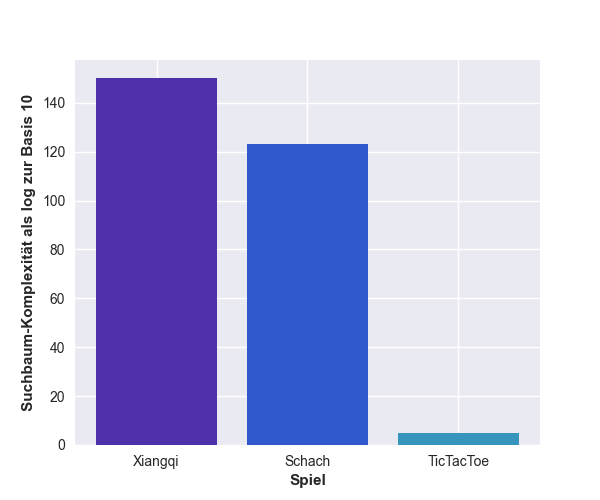
\includegraphics[width=\textwidth]{imgs/gameComplexity.png}
  \end{minipage}
  \hfill
  \begin{minipage}{0.49\textwidth}
    \centering
    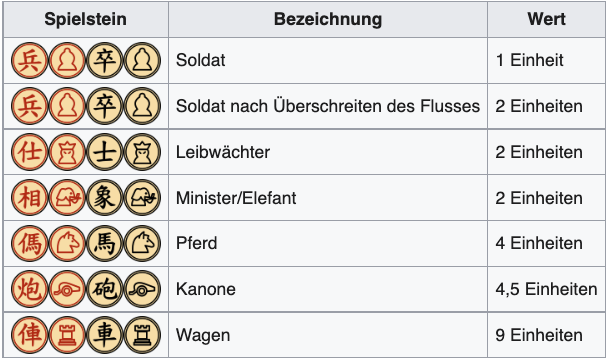
\includegraphics[width={\textwidth}]{imgs/Wert.png}
  \end{minipage}
  \captionsetup{justification=centering}
  \caption{Vergleich der Suchbaum-Komplexität von Xiangqi, Schach und TicTacToe (links) \\ Wert der Figuren (rechts)}
  \label{fig:compAndValue}
\end{figure}

\section{KI-Suche}
Die Suche in einer KI beschreibt den Prozess, unterschiedliche Züge zu spielen, diese zu bewerten und aus ihnen den besten Zug zu wählen. Hierfür hilft es, sich das Spiel als einen Baum-Datenstruktur mit Spielzuständen (en. state) {$s_{root}, s_2, s_3 ...$} als Knoten vorzustellen. Diese Knoten werden von Zügen {$a_1, a_2, a_3 ...$} als Zweige verbunden. Hierbei ist $s_{root}$ der Startzustand und alle untergeordneten Knoten beschreiben Positionen, die aus Folge von den Zügen entstehen. Diese Baum Datenstruktur wird auch \textit{Search Tree} bzw. \textit{Such-Baum} genannt. 
Wenn das Endergebnis des Spiels für jeden Zug bekannt wäre, bestünden die Bewertungen nur aus Verlust, Unentschieden und Sieg und die KI müsste nur einen Zug in die Zukunft schauen, um den Besten zu finden. In der Praxis ist kann jedoch aufgrund der unvorstellbar großen Such-Baum-Komplexität von Xiangqi ($10^{150}$) \ref{fig:compAndValue} der exakte Wert einer Position nicht ermittelt werden, weshalb dieser geschätzt werden muss.

\subsection{SHEF}
Genau dafür nutze ich eine \textit{Standard-Heuristic-Evaluation-Function (SHEF)}, die einen statischen Wert für jede Figur festlegt \ref{fig:compAndValue} und damit einen Spielzustand bewertet.
\textit{Piece-Square-Tables} implementierte ich, um diese Werte zu spezifizieren. Diese gehen von der Beobachtung aus, dass Figuren abhängig von ihrer Position unterschiedlich stark sind und geben demnach jeder Figur einen Feld-spezifischen Wert. Beispielsweise ist ein Turm vor dem gegnerischen Palast stärker als in einer Ecke. Eine großes Problem der SHEF, welches ich dabei erkannte, ist die absolute Abhängigkeit der Bewertung von den Positionen der Figuren und die fehlende Berücksichtigung der Brettstruktur, was zu großen Ungenauigkeiten führen kann (deshalb auch \textit{heuristisch}).

\subsection{Quiescene-Suche}
Betrachtet man folgendes Beispiel: \textit{„X steht auf einem starken Feld}, kann aber im nächsten Zug geschlagen werden", wird schnell klar, wie dies zu Problemen führen kann. Weil die SHEF nur die Position des Pferdes berücksichtigt und nicht sieht, dass das Pferd bedroht wird, implementierte ich eine \textit{Quiescene-Suche}, die eine Position so lange ausspielt, bis eine Position erreicht ist, wo keine Figuren geschlagen werden können. Somit sollen große Entscheidungsfehler behoben werden, indem nur Positionen ausgewertet werden, in denen der erste Teil des Beispiels zutrifft.
Ein weiteres Problem bleibt aber. Im Fall \textit{„X steht auf einem starken Feld, ist aber völlig umzingelt und damit stark eingeschränkt und weniger Wert"} , wird auch nach Einführung der Quiescene-Suche nur der erste Teil berücksichtigt und die Evaluation bleibt in vielen Fällen ungenau.
\begin{figure}
  \centering
  \begin{minipage}[b]{0.49\textwidth}
    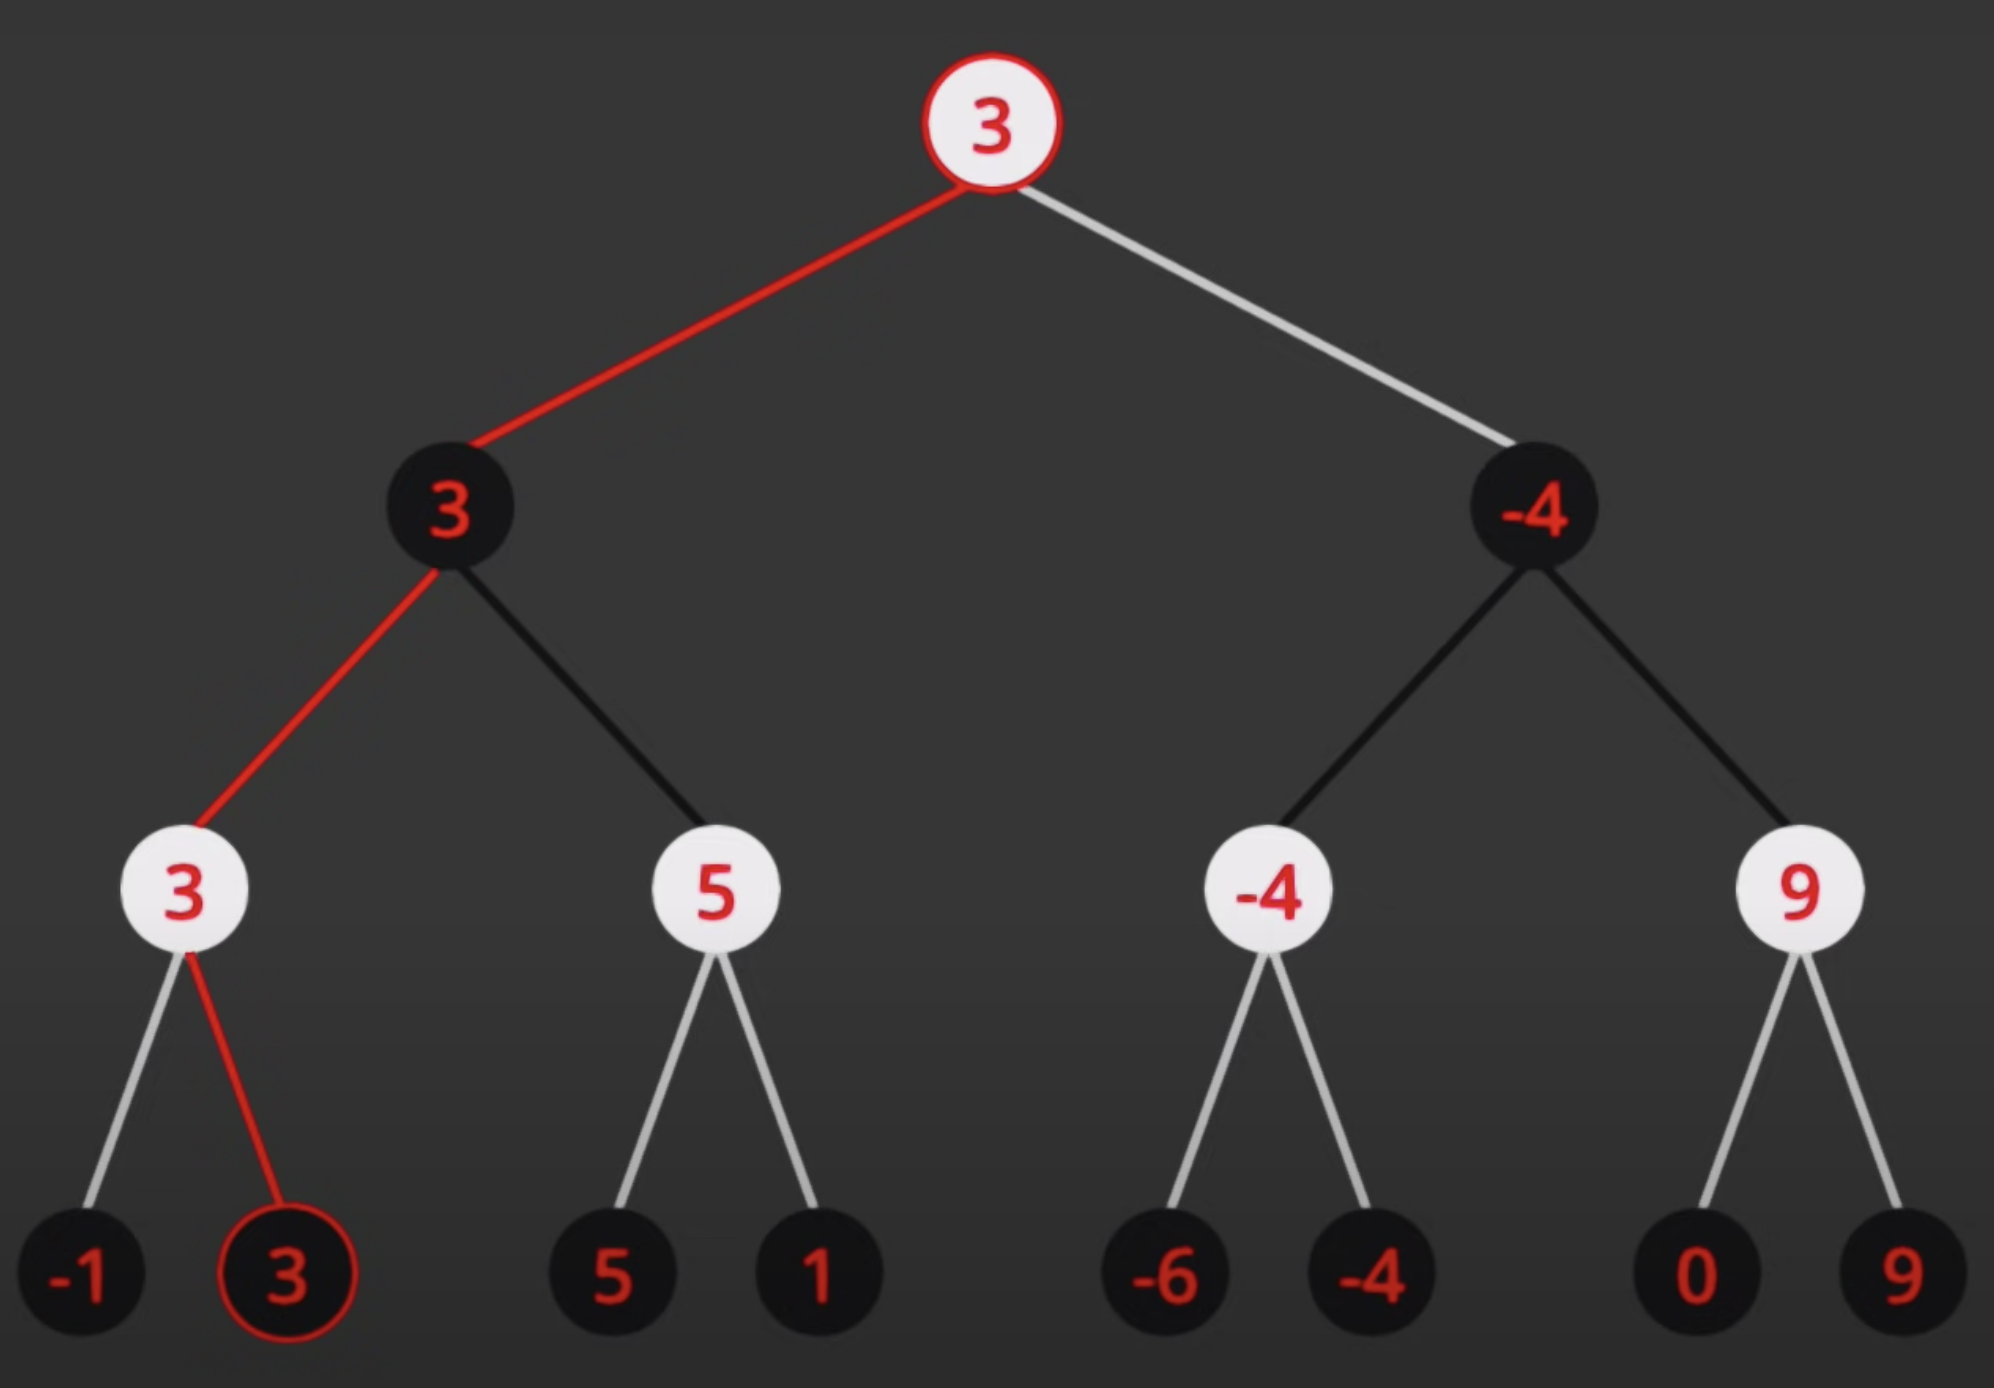
\includegraphics[width=\textwidth]{imgs/MM.png}
  \end{minipage}
  \hfill
  \begin{minipage}[b]{0.49\textwidth}
    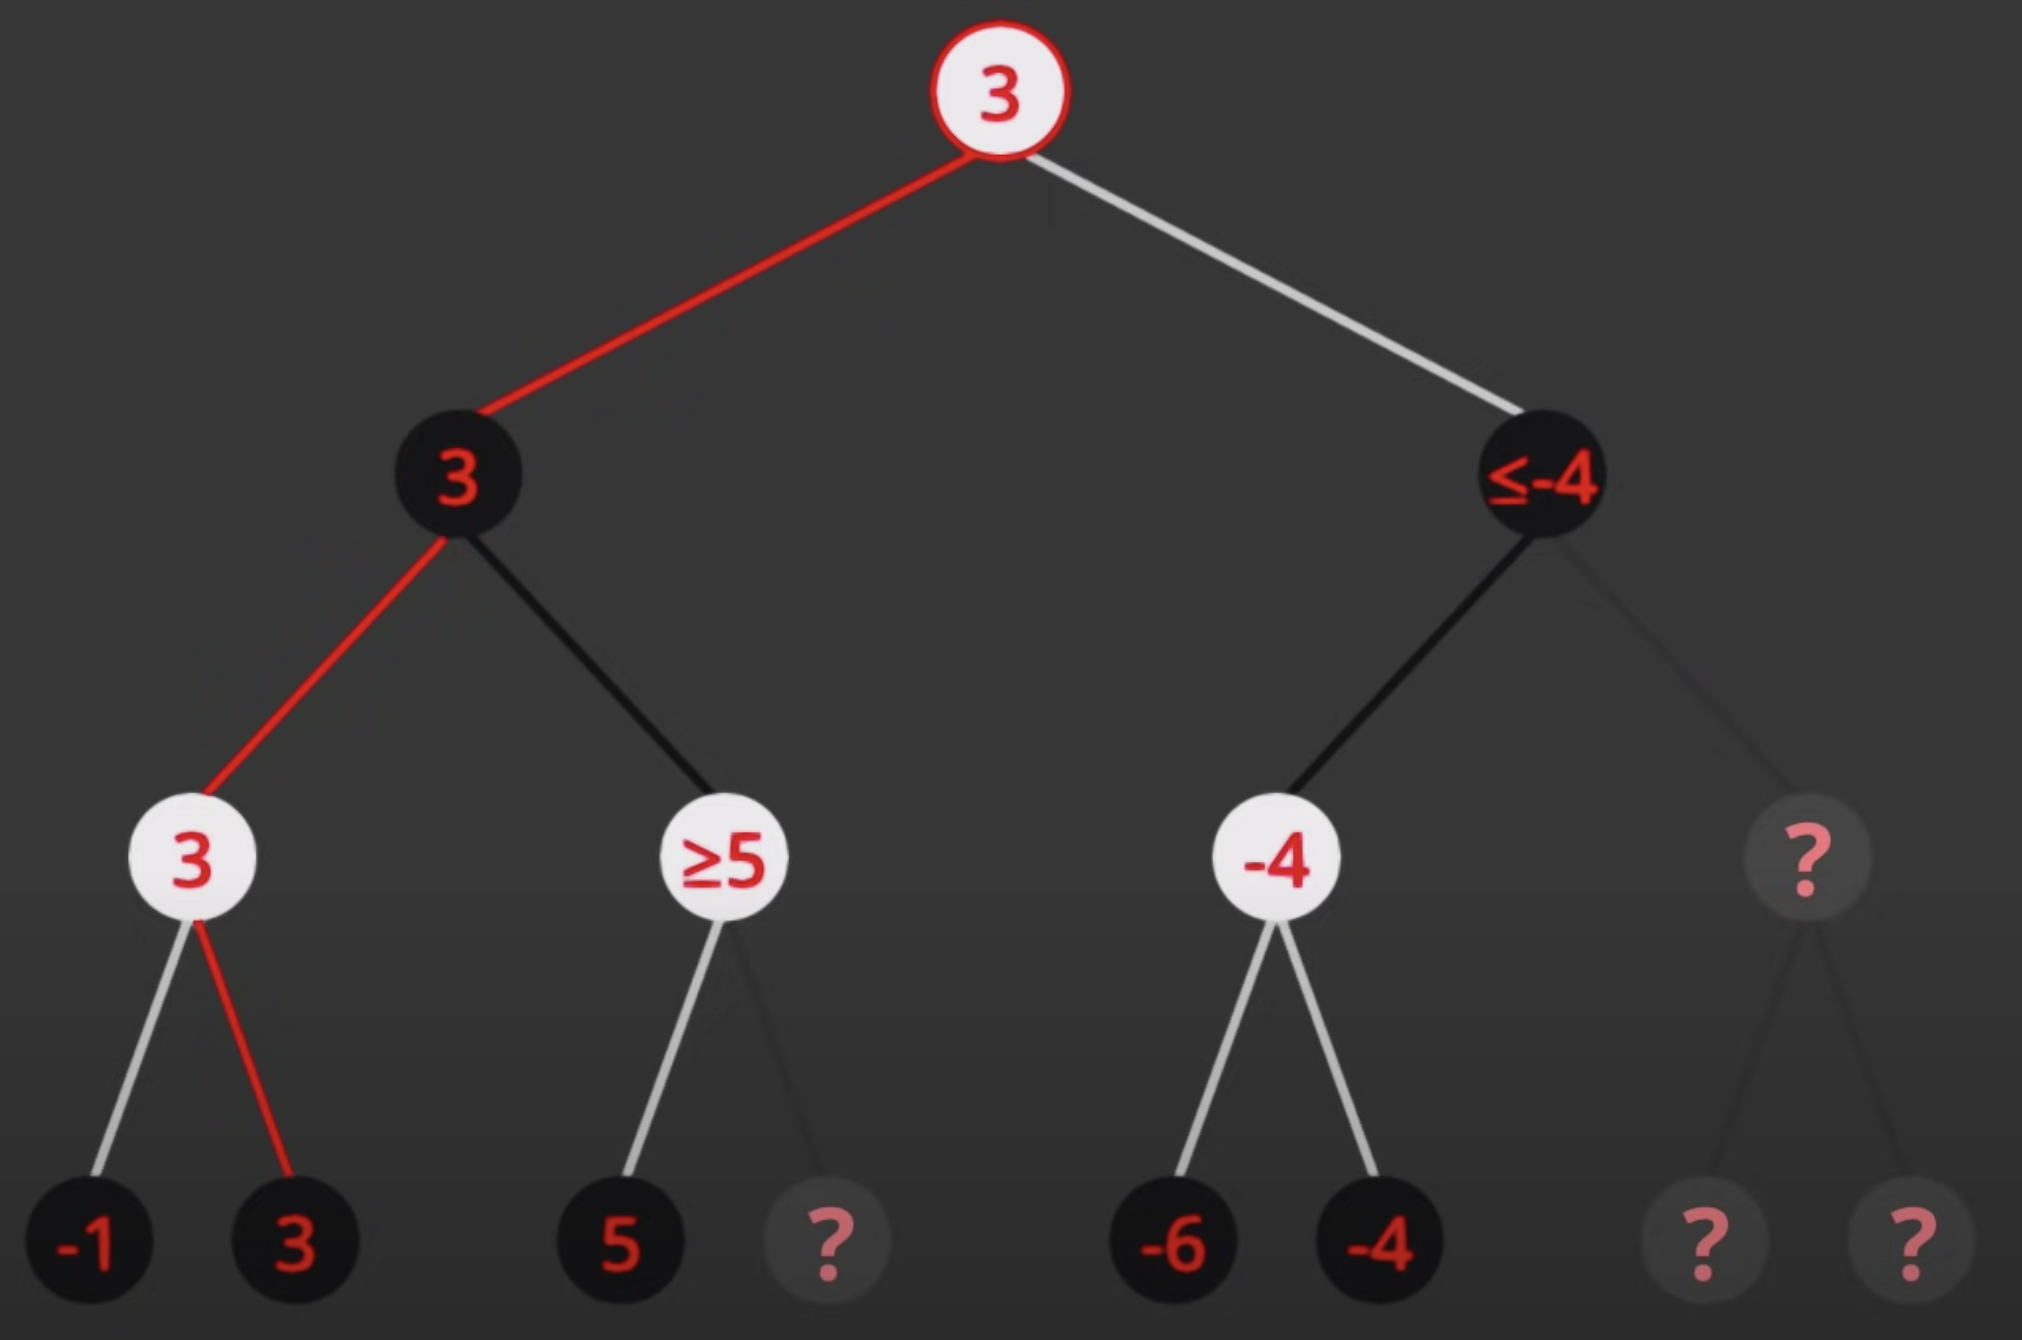
\includegraphics[width=\textwidth]{imgs/ABP.png}
  \end{minipage}
  \captionsetup{justification=centering}
  \caption{Einfache Visualisierung von Minimax. Weiß: max, schwarz: min (links) \\ Der gleiche Suchbaum, mit Alpha-Beta-Pruning (rechts)}
  \label{fig:mmabp}
\end{figure}

\subsection{MiniMax}
In meiner Recherche über einfache Spiel-KIs stieß ich auf den populären und weitverbreiteten MiniMax-Algorithmus \cite{mman} \ref{fig:mmabp}. Dieser ist zwar simpel und ineffizient, bildet aber das konzeptionelle Fundament selbst für Programme wie Stockfish.
Es wird angenommen, dass jeder Spieler an jeder Situation den optimalen Zug spielt. Das bedeutet, dass ein Spieler den erwarteten Gewinn laut der SHEF maximiert und der Gegner versucht, diesen zu minimieren. So werden die Blätter (unterste Knoten) des Such-Baums mit den Evaluationen der jeweiligen Positionen gekennzeichnet und die restlichen Knoten werden rekursiv durch Auswahl des Zuges mit dem höchsten (für max) bzw. dem niedrigsten (für min) Gewinn gekennzeichnet. Ich habe eine elegantere Methode genutzt, wo jeder Spieler den besten erreichten Wert seines Gegners mit -1 multipliziert, denn ein guter Wert aus Perspektive des Gegners ist ein schlechter Wert für sich selbst. Somit kann auf unterschiedliche Operationen basierend auf dem Spieler verzichtet und immer die \textit{max()} Funktion genutzt werden.

Ich implementierte diesen Algorithmus, erzielte jedoch nicht mein Ziel, hochperformante Algorithmen zu schreiben. Die Suche dauerte schon für drei Züge in die Zukunft rund zwanzig Sekunden. Dies lag daran, dass Minimax-Algorithmen eine exponentielle Zeit-Komplexität von $O(b^d)$ haben, wobei $b$ der Ausdehnungsfaktor und $d$ die Tiefe (en. depth) der Suche ist.

\begin{figure}
    \centering
    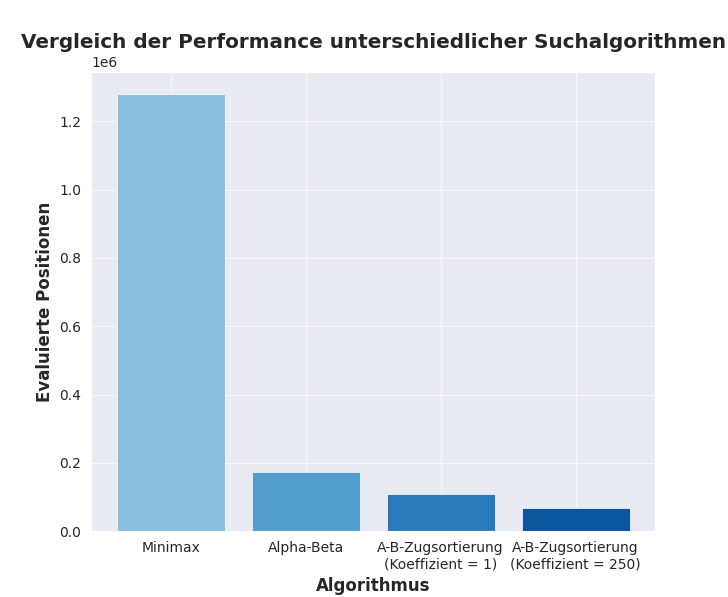
\includegraphics[width={0.5\textwidth}]{imgs/comp.png}
    \captionsetup{justification=centering}
    \caption{Evaluierte Positionen von jedem Algorithmus bei Suchtiefe von 4.
    Die Daten sind von jeweils 105 Suchen für jeden Algorithmus an unterschiedlichen Startpositionen gesammelt}
    \label{fig:comp}
\end{figure}

\subsection{Alpha-Beta-Pruning}
Ich fand heraus, dass Alpha-Beta-Pruning \cite{abp} die Leistung des Minimax-Algorithmus deutlich verbessert, indem es unbrauchbare Zweige des Such-Baumes frühzeitig abschneidet \ref{fig:mmabp}. Dies wird erreicht, indem für jeden Knoten im Baum zwei Werte, $\alpha$ und $\beta$, verwendet werden. $\alpha$ repräsentiert den besten Wert, den der aktuelle Spieler erreichen kann, und $\beta$ repräsentiert den besten Wert, den der gegnerische Spieler erreichen kann. Wenn $\alpha \geq \beta$ ist, wird der Rest des Zweigs abgeschnitten, da der Gegner den Knoten mit Wert $a$ nicht wählen wird und der aktuelle Spieler keine Möglichkeit hat, ein besseres Ergebnis zu erzielen.

Die Verwendung von $\alpha$ und $\beta$ ermöglicht es dem Algorithmus, schneller Entscheidungen zu treffen, indem unbrauchbare Zweige des Entscheidungsbaums und der damit verbundenen untergeordneten Baum-Struktur des Entscheidungsbaumes frühzeitig abgeschnitten werden. Dies führt zu einer signifikanten Reduzierung der Anzahl der Knoten, die untersucht werden müssen und damit zu einer deutlichen Leistungssteigerung. Die Untergrenze der Zeit-Komplexität liegt nur noch bei $\Omega(b^{d/2})$

\subsection{Zugsortierung}
Um die Anzahl der abgeschnittenen Zweige bei der Alpha-Beta-Suche zu maximieren, habe ich einen Zug Sortier-Algorithmus entwickelt. Dafür wird an jedem Knoten die Priorität jedes Zuges $a$ anhand des Wertes der sich bewegenden Figur $f$ und ggf. einer geschlagenen Figur $c$ bestimmt:
\[v_a = c_a * m - f_a\]
Hierbei ist $m$ eine Konstante, welche die Gewichtung des geschlagenen Figurenwertes kontrolliert. Ich fand heraus, dass die meisten Zweige abgeschnitten werden konnten, wenn $m \geq \dfrac{b}{w}$ ist ($b$ steht für den höchsten Wert unter allen Figuren, $w$ für den Schlechtesten). Somit hat selbst das Schlagen schlechter Figuren mit starken Figuren Vorrang über nicht-schlagende Züge. So wird z.B. ein Turm-schlägt-Bauern Zug vor einem Bauer-schlägt-Turm Zug erforscht, welcher wiederum Vorrang vor einem normalen Bauer-Zug hat.


\subsection{Multiprocessing und Parallelismus}
Um die Performance zu verbessern, verteilte ich den Algorithmus mit dem Multiprocessing Modul auf mehrere Prozessor-Kerne und konnte somit in acht Sekunden bis zu fünf Züge in die Zunkunft (\textit{133 Millionen} Positionen) suchen. 

\section{Autodidaktisches Reinforcement Learning}
Ich hätte die Alpha-Beta Suche noch lange weiter optimieren können, mir fehlte aber der Antrieb, weiterhin nur bereits existierende Konzepte zu verstehen und implementieren. Außerdem entdeckte ich während der Entwicklung entscheidende Schwächen der Alpha-Beta Suche.

Ich machte es mir demnach zum Ziel, einen weiteren großen Schritt zu gehen und dem Computer das Lernen zu Lehren. 

Zu Beginn hatte ich vor, große Datenbanken an Spielaufzeichnungen von Profis zu nutzen und damit ein neuronales Netzwerk zu trainieren. Das Problem war aber, dass diese nicht existieren, weshalb der Algorithmus selber in der Lage sein muss, diese Trainingsdaten zu generieren. Somit soll auch verhindert werden, dass das neuronale Netzwerk nur lernt, Menschen zu imitieren und kein neues Verständnis über das Spiel erlangt und eine Art Kreativität entwickelt. Zur Verfügung stehende Mittel sind dabei nur die Spielregeln. In anderen Worten: Etwa wie wir Menschen soll ein Deep Convolutional Neural Network durch eine Vielzahl von Spielen gegen sich selbst, tabula rasa, Xiangqi meistern. 

Dafür recherchierte ich über AlphaGoZero \cite{ag0} und AlphaZero \cite{a0} von Deepmind und fand heraus, wie es AlphaZero gelang, mit einem generischen Reinforcement Learning Algorithmus nur durch \textit{Self-Play} mehrere strategische Brettspiele zu meistern. Dies beseitigte vor allem das Bedürfnis zu professionellem Wissen und menschlicher Arbeit, um weitere domänenspezifischen Optimierungen zu treffen und löste weitere Probleme einer Minimax-basierten Suche.
Ich schaute mir Präsentationen an und  las den Forschungsbericht, in dem die grundsätzlichen Ideen grob beschrieben wurden. Es ist aber zu beachten, dass z.B. die Architektur des neuronalen Netzwerks und genauere Informationen zum Reinforcement Learning Algorithmus Geschäftsgeheimnisse sind und darüber hinaus klar angedeutet wurde, dass normale Hardware sie bei weitem nicht handhaben kann. Dieser Teil des Projekts erforderte sehr viel intensives Nachdenken, weil ich einerseits nur einen groben vorgegebenen Rahmen hatte und die Details in der Implementierung des Algorithmus selber erschließen und ihn darüber hinaus modifizieren musste, sodass er auf normaler Hardware lauffähig ist.

\begin{figure}
    \centering
    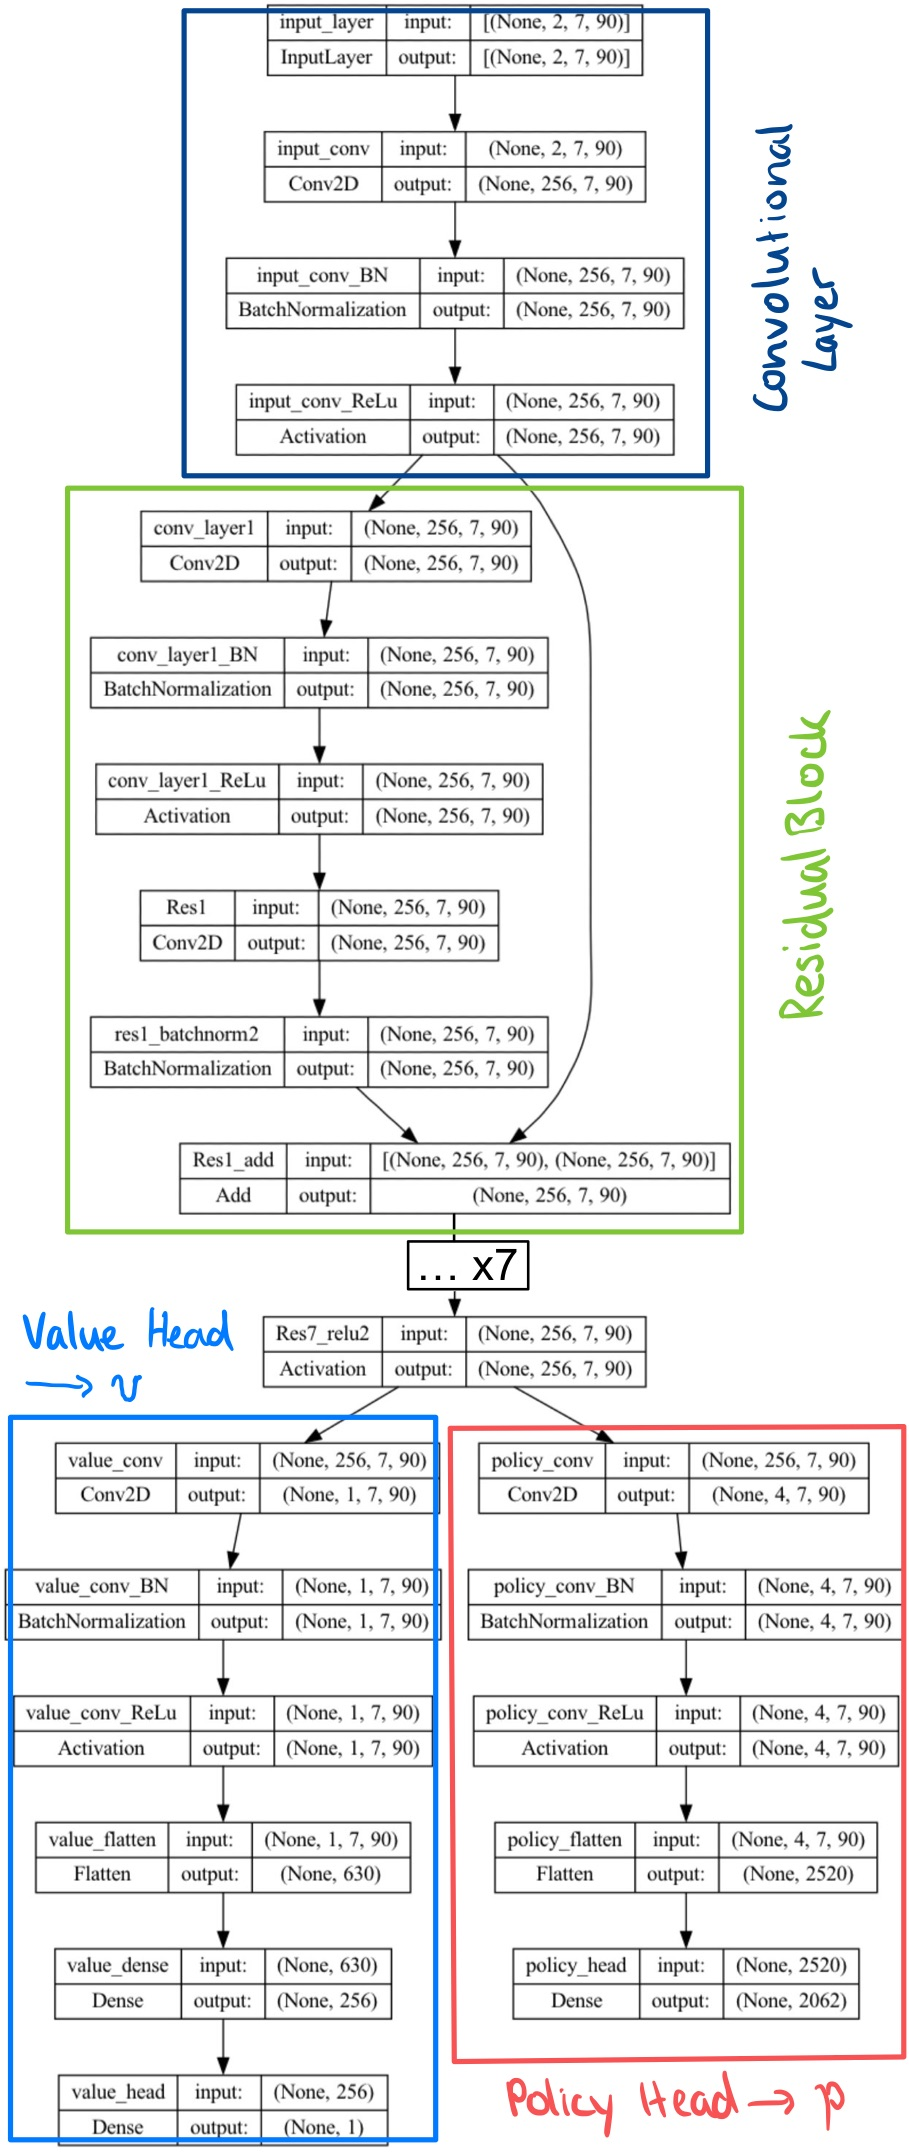
\includegraphics[width={0.63\textwidth}]{imgs/model.jpg}
    \caption{Neuronales Netzwerk visualisiert}
    \label{fig:model}
\end{figure}

\subsection{Modellarchitektur}
Um die bereits angesprochenen Probleme der SHEF zu lösen, entwarf ich ein Deep Convolutional Residual Neural Network mit tensorflow und keras, welches wie wir Menschen die Brettstruktur berücksichtigen soll und für normale Hardware gut geeignet ist. Hier war es wichtig, die Architektur möglichst klein zu halten, gleichzeitig aber so groß zu lassen, dass es lernfähig ist (\textit{„So klein wie möglich, so groß wie nötig}). Mathematisch sieht es wiefolgt aus:
\[(p, v) =  f_\theta(s)\]Eingabe ist die Brettposition $s$, Ausgabe ein Vektor einer Wahrscheinlichkeitsverteilung $p$ über alle Züge in der Action Space und ein Skalar $v$ zwischen -1 (Niederlage) und 1 (Sieg), der das erwartete Ergebnis von Position $s$ schätzt. Das Netzwerk lernt die optimalen Parameter $\theta$. Es lernt in anderen Worten also, wie gut bestimmte Züge in einer bestimmten Position sind und den Wert der Position selbst zu schätzen. 
Meine Architektur besteht aus zwei Hauptkomponenten:
\begin{enumerate}
\item Ein Convolutional Layer. Diese sind generell besonders gut für Erkennung räumlicher Hierarchien und Muster, ähnlich wie das menschliche visuelle System. Der Convolutional Layer nimmt den aktuellen Brettzustand als Eingabe und gibt eine Reihe von Merkmalen aus, die das Brett repräsentieren.
\item Ein Multi-Layer Perceptron (MLP), das die Ausgabe vom Concvolutional Layer als Eingabe nimmt und neben dem geschätzten Wert des Spielzustandes $v$ eine Wahrscheinlichkeitsverteilung $p$ über alle möglichen Züge ausgibt. Das MLP besteht aus sieben Residual Layers, einem \textit{value head} (für den Wert $v$) und einem \textit{policy head} (für die Wahrscheinlichkeitsverteilung $p$). 
\end{enumerate}
Residual-Schichten ermöglichen es dem Netzwerk statt der Ausgabe den Residual, also den Unterschied zwischen Eingabe und gewünschter Ausgabe, zu lernen. Dadurch wird das Problem des verschwindenden Gradienten behoben. Residual-Schichten erleichtern auch das Training sehr tiefer Netzwerke, da sie es ermöglichen, neue Schichten hinzuzufügen, ohne die Leistung zu verschlechtern. 

\subsection{MCTS}
Die Implementierung des Monte-Carlo Tree Search (MCTS) Algorithmus \cite{mcts} wird aus gleichen Gründen wie beim Zuggenerator abstrahiert. Wichtig ist, dass die Suche eine neue, informierte und somit genauere Wahrscheinlichkeitsverteilung $\pi$ mithilfe des aktuellen CNN $f_\theta$ generiert, welche dann genutzt werden, um die Parameter $\theta$ anzupassen. Ich habe mir erschlossen, dass MCTS auf der Idee basiert, den menschlichen Gedankenverlauf zu simulieren.

Der Algorithmus besteht aus vier Schritten: Auswahl, Erweiterung, Simulation und Backpropagation.
\begin{enumerate}

\item Auswahl: Im ersten Schritt wird der Algorithmus durch den aktuellen Zustand des Spiels navigieren und den Zug auswählen, der die höchste geschätzte Siegchance hat.

\item Erweiterung: Sobald ein Blattknoten erreicht ist, wird dieser mit untergeordneten Knoten erweitert, die erlaubte zukünftige Zustände des Spiels repräsentieren.

\item Simulation: Der Algorithmus bestimmt dann die Wahrscheinlichkeit, dass der ausgewählte Zug zum Sieg führt. Hierfür wird die Wert-Ausgabe $v$ vom Neuronalen Netzwerk genutzt.

\item Backpropagation: Schließlich wird das Ergebnis der Simulation entlang des im Suchbaum gegangen Weges zurückprogagiert, um die geschätzte Siegchance für jeden besuchten Knoten im Entscheidungsbaum zu aktualisieren.
\end{enumerate}

\subsection{Augmentation von Trainingsdaten}
Nachdem ich das Grundprinzip des selbstlernenden Algorithmus  implementiert hatte, bekam ich die Idee, die Bitboards und Züge immer an die Perspektive eines  Spielers anzupassen.
Dadurch wurde die Anzahl der Labels, also der Größe der CNN-Ausgabe verringert, da einige Züge nach perspektivischer Anpassung äquivalent sind, z.B. ist [89, 71] aus Perspektive eines Spielers äquivalent zu [0, 18] aus Perspektive des Anderen. Diese Methode ist menschennäher und sorgt für reduzierte Modellkomplexität, schnelleres Lernen und erhöhte Performance. Viel wichtiger ist aber, dass so allgemeinere Muster erkannt, standardisierte Trainingsdaten gesammelt und Verwirrung beim Training durch unterschiedliche Wertungen perspektivisch äquivalenter Züge vermieden werden können. Auch ist somit kein “side plane” mehr als Eingabe erforderlich, um die sich bewegende Seite anzugeben und die Eingabe ist komplett für die Erkennung von Mustern auf dem Brett optimiert. Ein weiterer wichtiger Vorteil ist die Augmentation von Trainingsdaten um 200\%, weil für jede Position aus beiden Perspektiven ein Trainingsbeispiel gesammelt werden kann.

Ich erkannte außerdem, dass die Effektivität der Sammlung von Trainingsdaten um weitere 200\% gesteigert werden kann, indem die Symmetrie des Bretts ausgenutzt wird, um die Bitboards entlang der y-Achse zu spiegeln. Somit kann jeder Spielzustand in ein Set aus vier Trainingsbeispielen umgewandelt werden.


\subsection{Training}
Traingsdaten werden durch Spiele gegen sich selbst mit MCTS gesammelt. Im ersten Schritt vom MCTS (Auswahl) wird mithilfe von Dirichlet Noise für einen gewissen Grad an Zufall gesorgt, sodass nicht immer deterministisch der beste Zug gewählt wird, sondern der Suchbaum erforscht wird, um zukünftige gute Positionen zu entdecken, die aus nicht so guten Zügen (laut des CNN) entstehen. 
Am Ende jedes Spiels wird jedes Trainingsset mit dem Endergebnis $z$ ergänzt, sodass neben der verbesserten Wahrscheinlichkeitsverteilung $\pi$ auch die Bewertung der Positionen genauer sind. Das Ziel vom Training ist es, die Differenz zwischen vorhergesagtem Ergebnis $v$ und Endergebnis $z$ zu minimieren und die Ähnlichkeit zwischen vorhergesagter Wahrscheinlichkeitsverteilung $p$ und $\pi$ zu maximieren, sodass das Netzwerk $f_\theta$ immer genauere Vorhersagen treffen kann.
Hierfür nutze ich den SGD (Stochastic Gradient Descent) Optimierer \cite{sgd} und eine Verlust-Funktion $l$, welche mean-squared-error (MSE) für die Ergebnisse und categorical-cross-entropy \cite{crossentropy} für die Wahrscheinlichkeitsverteilung nutzt. Mathematisch notiert sieht diese wiefolgt aus:
\[
l = (z - v)^2 - \pi^T \log p + c\lVert \theta \rVert^2
\]
Das $T$ steht für \textit{Transpose}, eine Matrizen-Operation, die benutzt wird, um die Dimensionen für eine Matrizen-Multiplikation anzupassen.

\section{Alpha-Beta-Zero}
Nun habe ich bereits zwei komplett unterschiedliche Algorithmen implementiert.

Während sich AlphaZero also auf die in den letzten Jahren erst entdeckte Macht des maschinellen Lernens verlässt, bringt Stockfisch alte Techniken an ihre Grenzen. In meiner Recherche fand ich heraus, dass die unterschiedlichen Methoden für sehr viel Uneinigkeit und Zerspaltung zwischen KI-Forschern und Schach-Enthusiasten führte.

Vielleicht war es die fehlende Voreingenommenheit meinerseits zusammen mit der Erkennung der Schwächen beider Methoden, welche mich zu der Entdeckung ihrer Kompatibilität führten, bevor ich sie überhaupt vergleichen konnte (einer meiner vorherigen Ziele).

Alpha-Beta-Zero ist der Teil von Algorithmus, in der ich Alpha-Beta-Suche und den von AlphaZero inspirierten selbstlernenden Reinforcement Learning Algorithmus kombiniere. Ich entwickelte mehrere Ideen, um dies zu tun und entschied mich am Ende für die effizienteste, einfachste und eleganteste Methode. Dabei führe ich beide Algorithmen parallel aus, ermittele einfach den ausgewählten Zug beider Algorithmen und addiere ihren Wert laut den Evaluationen beider Such-Algorithmen, um am Ende den Zug auszuwählen, der $V$ maximiert.
\begin{equation}
    V = \pi_a \times m + \beta_a
\end{equation}
Die Evaluationen beider Algorithmen sind $\pi$ für MCTS, $\beta$ für die Alpha-Beta-Suche und $a$ ist ein Zug. Der Koeffizient $m$ kontrolliert dabei die Gewichtung der MCTS-Evaluationen und steht somit proportional zur Autonomie des Neuronalen Netzwerks, sodass der Algorithmus sich in einem frühen Stadium des CNN bei einem niedrigem $m$-Wert größtenteils auf die Alpha-Beta Suche verlässt. Im Gegenteil wird bei einem leistungsstarken CNN mit viel Training mithilfe eines hohen $m$-Werts nur bei offensichtlichen Entscheidungsfehlern vom MCTS, z.B. bei starkem vorhergesehenen Materialverlust oder einem Matt, eine Änderung des Zuges vorgenommen. 

Alpha-Beta-Zero ist ein Hybrid aus zwei sehr unterschiedlichen Algorithmen, der die Schwächen einer Methode mit den Stärken der anderen ausgleicht. 

\begin{figure}
  \centering
  \begin{minipage}[c]{0.33\textwidth}
    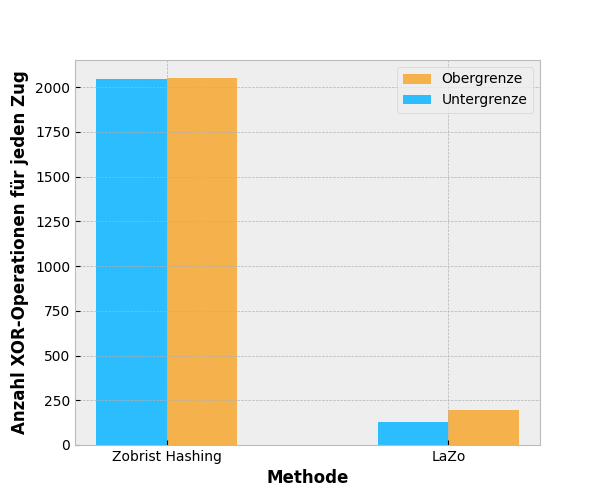
\includegraphics[width=\textwidth]{imgs/zobristComp.png}
  \end{minipage}
  \hfill
  \begin{minipage}[c]{0.33\textwidth}
    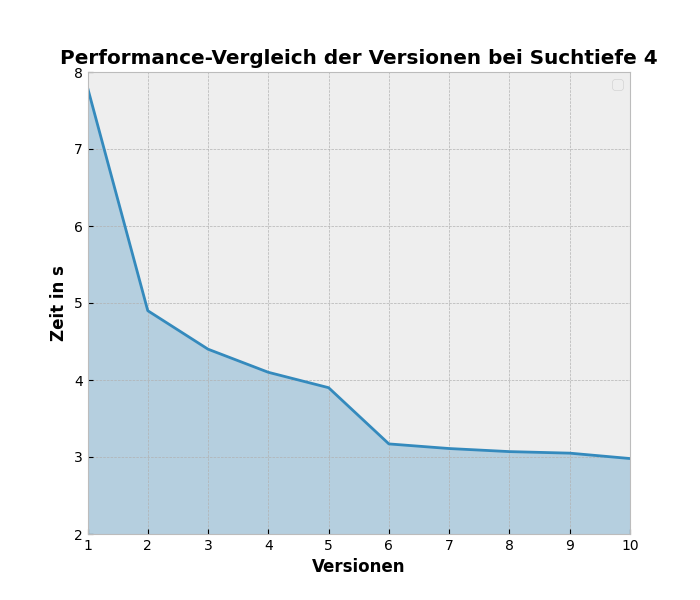
\includegraphics[width=\textwidth]{imgs/Perft.png}
  \end{minipage}
  \hfill
  \begin{minipage}[c]{0.32\textwidth}
      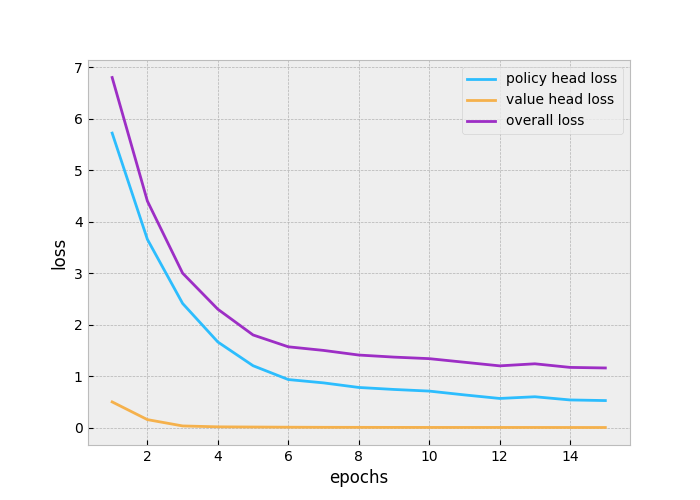
\includegraphics[width={\textwidth}]{imgs/loss.png}
  \end{minipage}
  \captionsetup{justification=centering}
  \caption{Vergleich der Berechnungen von Zobrist-Hashing und LaZo (links) \\ Performance-Vergleich unterschiedlicher Versionen des Zuggenerators bei Suchtiefe 4 (mittig) \\ Die Loss-Werte im Laufe von 15 Trainings-Epochen mit 800+ Trainingsbeispielen (rechts)}
  \label{fig:results}
\end{figure}

\section{Ergebnisse}
Nach gut acht Monaten und vielen Iterationen von Recherchieren, Nachdenken, Ausprobieren, Scheitern und wieder Recherchieren gelang es mir, eine Xiangqi-KI zu entwickeln, die einen selbstlernenden Algorithmus mit der traditionellen Alpha-Beta-Suche harmonisch ergänzt. 

Dafür entwickelte ich selber eine Xiangqi-Applikation. Dabei entwarf ich eine neue Methode, um Zobrist-Hashing um bis zu 1600\% zu verbessern \ref{fig:results}. Mein Zuggenerator ist mittlerweile die schnellste Python-Implementierung weltweit und kann bei Performance-Tests auf meinem Laptop (M1 Pro Chip, acht Kerne, 16GB RAM) bis zu $1.080.000$ Blätter pro Sekunde im Suchbaum erreichen \ref{fig:results}. Diese Performance-Tests (perft) werden durchgeführt, um die Leistung des Zuggenerators zu ermitteln und seine Genauigkeit durch den Vergleich mit dem Konsens anderer Programme zu überprüfen. Diese stimmen zu 100\% überein. 

Ich entwickelte einen domänenspezifisch optimierten Alpha-Beta-Suchalgorithmus, welcher in ca. acht Sekundenbis zu fünf Züge (~133.000.000 Blattknoten) in die Zukunft schauen kann.

Im Reinforcement Learning Algorithmus konnten durch Anpassungen der Modellarchitektur-Komplexität die benötigte Hardware von 5000+ TPUs auf einen Laptop reduziert werden. Die Modifizierung Eingaben des neuronalen Netzwerks erleichterte dies und erlaubte kombiniert mit der Ausnutzung von Symmetrien des Bretts eine Augmentation der Trainingsdaten um 400\%. Die Generation von vier Trainingssets dauert dadurch nicht mehr als drei Sekunden und das Training verläuft reibungslos auf einer einzelnen GPU \ref{fig:results}.

% Ohne viel Training schlägt Alpha-Beta-Zero mittlerweile bereits die zweitbeste KI auf Xiangqi.com und hält auch bei dem „Endboss" lange mit.
\section{Ausblick}
Das Projekt befindet sich derzeit immer noch im Entwicklungsstadium. Zurzeit arbeite ich an einem sogenannten Elo-System zur Evaluation meiner Alpha-Beta-Zero Methode. So kann die Spielstärke der KI gemessen und seine Entwicklung analysiert werden, damit ich anschließend die Hyperparameter für den Trainingsprozess optimieren kann.

Der Zuggenerator ist nach zahlreichen Optimierungen zwar schon hochperformant, besitzt aber noch weiteres Potenzial für Steigerungen der Performance durch Just-in-time-Kompilierung mithilfe von Bibliotheken wie numba. Auch die Alpha-Beta-Suche kann weiter verbessert werden, etwa mit Methoden wie iterative deepening, transposition tables und der Optimierung vom Parallelismus.

Ein weiterer interessanter Schritt, den man zukünftig gehen könnte, ist die Modifizierung eines echten Bretts, sodass die KI mithilfe eines Microcontrollers ein eingebautes mechanisches Konstrukt unter dem Brett steuern kann, um die Entscheidungen der KI in echte Züge auf einem physischen Brett zu übertragen.

\section{Zusammenfassung}
Zusammengefasst konnte ich die benötigte Hardware innovativer Algorithmen auf normale Konsumenten anpassen, indem ich diesen mit einem hochoptimierten traditionellen Suchalgorithmus ergänzte, entwickelte dafür eine hochperformante Xiangqi-Applikation und entwarf neue Konzepte und Algorithmen. Dafür musste ich zahlreiche mathematische Konzepte verstehen und mein algorithmisches Denken an die Grenzen bringen. 

Ich habe realisiert, dass neue Konzepte oft durch die Kombination von Neu und Alt, durch die Erweiterung von innovativen Konzepten und traditionell anerkannten Methoden, entstehen.

Ich lernte auch, dass diese neuen Konzepte nur durch kritisches Hinterfragen und intensiver Beschäftigung mit den herkömmlichen Methoden entsteht und oft sehr viel Mut und eine Bereitschaft zum Scheitern erfordert. Meine Perspektive zu Bugs und ungeplantem Verhalten des Programms änderte sich und ich fing an sie nicht als Scheitern, sondern als Versuche zu sehen.  

Es war ein langer Prozess vom wiederholten Kopfzerbrechen und Scheitern, der mir beibrachte, dass das Verstehen von komplexen Themen manchmal vielleicht gar nicht so unmöglich ist wie es scheint. Mit etwas Bescheidenheit, der Akzeptanz des eigenen Unwissens und sehr viel Offenheit zum Lernen kann man diese Konzepte nicht nur verstehen und umsetzen, sondern auch erweitern, auf Ihnen aufbauen, vielleicht anderen Menschen helfen und auf dem Weg zu einem besseren Informatiker werden.

\newpage

\printbibliography
% \section{Quellen- und Literaturverzeichnis}
% \url{https://github.com/Simuschlatz/CheapChess}, 15.01.23, Simon Ma, CheapChess Quellcode für detaillierte Beschreibungen der angewandten Methoden
% \\
% \url{https://www.chessprogramming.org/Main_Page}, 15.01.23, 
% Chessprogramming Wiki, Wikipedia für Schachprogrammierung
% \\
% \url{https://en.wikipedia.org/wiki/Monte_Carlo_tree_search}, 15.01.23, Wikipedia, Monte-Carlo-Tree-Search
% \\
% \url{https://de.wikipedia.org/wiki/Xiangqi}, 15.01.21, Wikipedia, Xiangqi
% \\
% \url{https://www.xiangqi.com/}, 15.01.23, Xiangqi.com, Play Chinese Chess For Free on the \#1 Xiangqi Site!
% \\
% \url{https://www.deepmind.com/}, 15.01.23, Deepmind, Tocherfirma von Google
% \\
% \url{https://arxiv.org/abs/1712.01815}, Deepmind, Mastering Chess and Shogi by Self-Play with a General Reinforcement Learning Algorithm
% \\
% \url{https://www.youtube.com/c/SebastianLague}, 15.01.23, Sebastian Lague
% \\
% \url{https://www.youtube.com/watch?v=l-hh51ncgDI}, 21.08.22, Sebastian Lague, Algorithms Explained – minimax and alpha-beta pruning
% \\
% \url{https://en.wikipedia.org/wiki/Game_complexity} 15.09.22, Wikipedia, Game complexity
\end{document}